\selectlanguage{german}
%-----------------------------------------------------------------------------
\chapter{Umsetzung}\label{chap:Umsetzung}
%-----------------------------------------------------------------------------
\chapterstart
In diesem Kapitel wird die Umsetzung der Anforderungen in die Software erläutert. Es werden dabei besonders die Aspekte der Datenpersistenz, der Concurrency und der Skalierbarkeit vorgestellt.
\section{Überblick und Architektur}
Ausgehend von den Anforderungen wurde die Umsetzung des Schedulers\footnote{Die Umsetzung erfolgte unter dem Namen \textit{dJob}.} in Verantwortlichkeiten geteilt:
\begin{enumerate}
	\item Die Start-Prozedur
	\item Die \textit{Worker} die die Umsetzung der Aufgaben übernehmen
	\item Das Ausführen der Aufgaben \textit{Job} und planen der nächsten Ausführungszeit - der \textit{Scheduler}
	\item Das Laden von Aufgaben - der \textit{JobLoader}
\end{enumerate}
Die Trennung der Umsetzung erfolgte für den Scheduler und den JobLoader durch Interfaces gekapselt (siehe \ref{fig:architecture}). Die Instanziierung der tatsächlichen Klassen erfolgt zur Laufzeit über \textit{dependency injection}\cite{fowler2004}. Damit können diese Teile ausgetauscht werden und in etwa der Scheduler durch einen Echtzeit-fähigen Scheduler ausgetauscht werden ohne am Code selbst etwas ändern zu müssen\footnote{Die Umsetzung der injection dependency erfolgt in der Klasse \textit{ObjectRepository} ebenso um Rahmen dieser Arbeit. Umgesetzt wurde eine von außen konfigurierbare, explizite injection, einem \textit{service locator} nach Fowler. Verwendet wird diese mittels \textit{var service = ObjectRepository.Get<ServiceType().}}.
\begin{figure}
	\centering
	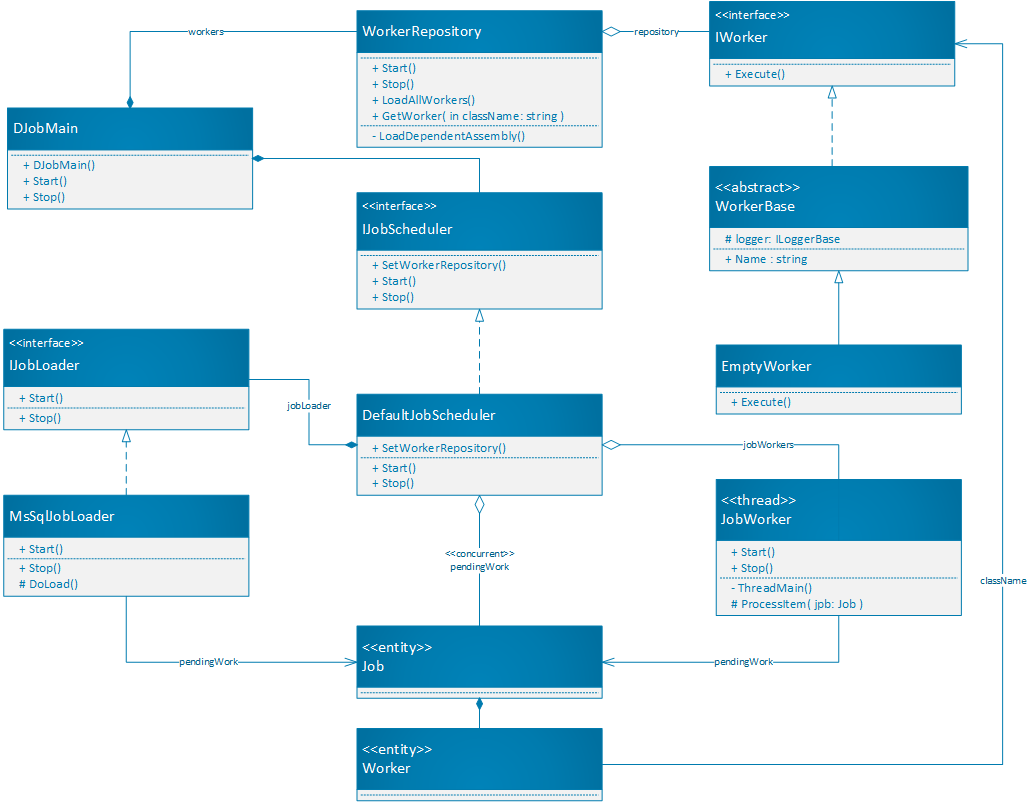
\includegraphics[width=0.7\linewidth]{images/architecture.png}
	\caption{Architekturübersicht des Schedulers, eigene Darstellung}
	\label{fig:architecture}
\end{figure}
\\
\section{Datenbank}
asdasd
\subsection{Datenbankmodell}
aasdas
\subsection{Zugriff}
sdasdaas
\section{Skalierung}
sdfsfs
\subsection{Skalierung der Leistung}
sdsds
\subsection{Funktionale Skalierung}
sdsd
\begin{lstlisting}[caption={Dynamic Loading, siehe WorkerRepository.cs - LoadAllWorkers()},label={lst:dynamicloading},captionpos=b]
foreach ( string file in  workerDirectory.GetFiles( "*.dll" ) )
{
	Assembly assembly = Assembly.LoadFile( file );

	foreach ( Type typeToLoad in assembly.GetTypes()
					.Where( t => t.ImplementsInterface<IWorker>() ) )
	{
		IWorker w = (IWorker)Activator.CreateInstance( typeToLoad );

		w.Initialize( ObjectRepository.Get<IConfigurationProvider>( ), logger );

		if( ! repository.TryAdd( typeToLoad.FullName, w ) )
		{
			throw new InvalidOperationException
			( $"Could not add class '{typeToLoad.FullName}' to repository");
		}
	}
}
\end{lstlisting}
\section{Concurrency}
dasdasd
\subsection{Threadpool}
asda
\subsection{Producer-Consumer}
adadsa
\subsection{Blocking-Queue}
\lstlistingname{ BlockingQueue-V1}
\begin{lstlisting}
	    /// <summary>
	/// own, experimental, implementation of ablocking, notifying Q for a producer/ consumer model
	/// </summary>
	public class MyBlockingQueueV1<T>
	{
		/// <summary>
		/// The backing store used for the elements
		/// </summary>
		private Queue<T> backingStore = new Queue<T>();
		
		/// <summary>
		/// lock to protect the q
		/// </summary>
		private object myLock = new object();
		
		
		
		public MyBlockingQueueV1()
		{ /* empty */ }
		
		public void Enque( T newElement )
		{
			lock ( myLock )
			{
				backingStore.Enqueue( newElement );
			}
		}
		
		
		public T Dequeue()
		{
			lock ( myLock )
			{
				return backingStore.Dequeue();
			}
		}
		
		public T TryDequeue()
		{
			lock( myLock )
			{
				if( !IsEmpty() )
				{
					return Dequeue();
				}
				else
				{
					return default( T );
				}
			}
		}
		
		public bool IsEmpty()
		{
			lock ( myLock )
			{
				return backingStore.Count == 0;
			}
		}
	}
\end{lstlisting}
\section{Verbesserungsmöglichkeiten}
\chapterend
